% Start point: Porter model Author: Charles-Axel Dein URL: http://www.texample.net/tikz/examples/porter-model/
\documentclass[10pt,a4paper]{article} 

\usepackage[hmargin=1cm,vmargin=1.5cm]{geometry}
\renewcommand{\rmdefault}{bch} % change default font

\usepackage[english]{babel}
\usepackage[utf8]{inputenc}
\usepackage{tikz} 
\usetikzlibrary{arrows,decorations.pathmorphing,backgrounds,fit,positioning,shapes.symbols,chains}

\begin{document}

%\begin{figure}[h]
%\centering
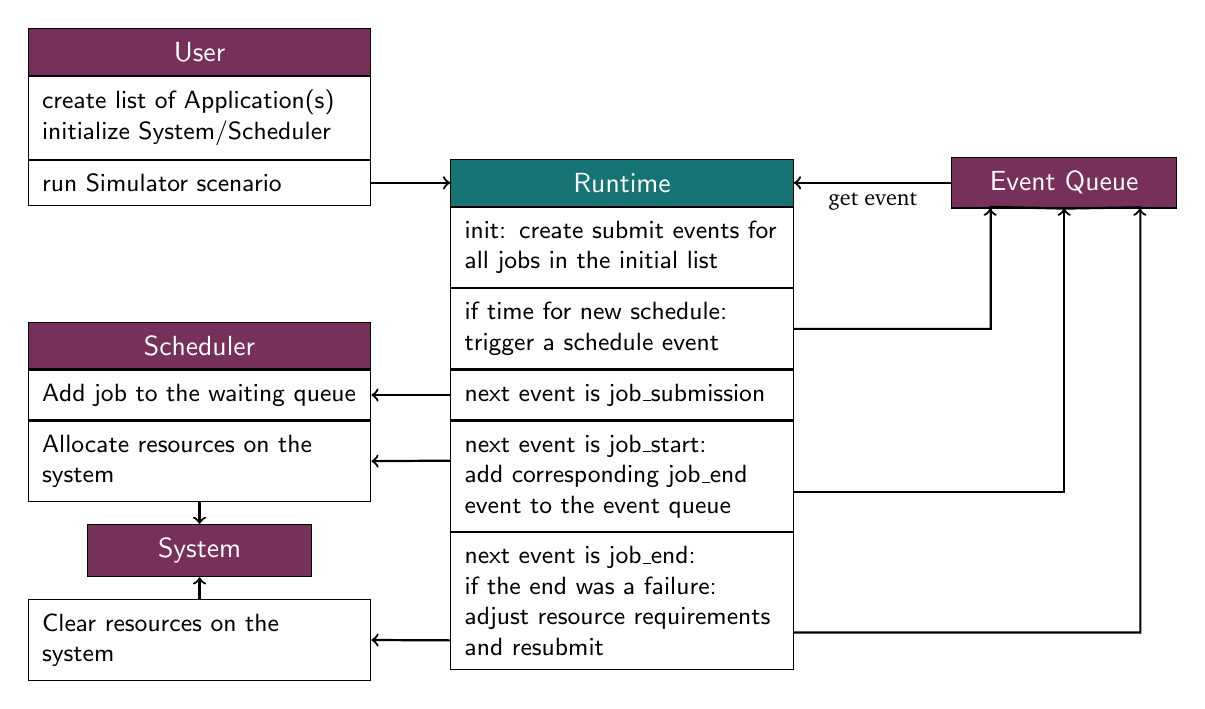
\begin{tikzpicture}
[node distance = 0.5cm, auto,font=\footnotesize,
% STYLES
every node/.style={node distance=3cm},
% The comment style is used to describe the methods of each class
user/.style={rectangle, draw, inner sep= 5pt, text width=4cm, node distance=0.25cm, font=\small\sffamily},
comment/.style={rectangle, draw, dashed, inner sep= 5pt, text width=4cm, node distance=0.25cm, font=\small\sffamily},
% Define styles for each type of class
api/.style={rectangle, draw, fill={rgb:red,31;green,164;blue,163}, inner sep=5pt, text width=4cm, text badly centered, minimum height=0.2cm, text=white, font=\sffamily},
internal/.style={rectangle, draw, fill={rgb:red,96;green,39;blue,73}, inner sep=5pt, text width=4cm, text badly centered, minimum height=0.2cm, text=white, font=\sffamily}] 


% User
\node [internal] (user)  at (0, 0) {User};
\node [user, below=0 of user] (user-desc) {create list of Application(s)\\
initialize System/Scheduler};
\node [user, below=0 of user-desc] (user-create) {run Simulator scenario};

\node [api, right=1cm of user-create] (simulator) {Runtime};
\node [user, below=0 of simulator] (sim-init) {init: create submit events for all jobs in the initial list};
\node [user, below=0 of sim-init] (sim-trigger) {if time for new schedule:\\ trigger a schedule event};
\node [user, below=0 of sim-trigger] (sim-submission) {next event is job\_submission};
\node [user, below=0 of sim-submission] (sim-start) {next event is job\_start:\\ add corresponding job\_end event to the event queue};
\node [user, below=0 of sim-start] (sim-end) {next event is job\_end:\\ if the end was a failure:\\ adjust resource requirements and resubmit};

\node [internal, right=2cm of simulator, text width=2.5cm] (eventq) {Event Queue};

\node [user, left=1cm of sim-submission] (sch-add) {Add job to the waiting queue};
\node [internal, above=0 of sch-add] (scheduler) {Scheduler};
\node [user, below=0 of sch-add] (sch-allocate) {Allocate resources on the system};

\node [internal, below=0.28cm of sch-allocate, text width=2.5cm] (system) {System};

\node [user, below=0.28cm of system] (sch-clear) {Clear resources on the\\system};

%%%%%%%%%%%%%%%%

\path[->,thick] 
(user-create) edge (simulator)
(eventq) edge node[auto] {get event} (simulator)
(sim-submission) edge (sch-add)
(sch-allocate) edge (system)
(sch-clear) edge (system);

\draw[->,thick] (sim-trigger.east) -| ++(2.5,0) -- ++(0,1.55) -- (eventq.south)+(-9.4mm,0);	
\draw[->,thick] (sim-start.east)+(0,-2mm) -| (eventq.south);
\draw[->,thick] (sim-end.east)+(0,-4mm) -| ++(4.4,0) -- ++(0,5) -- (eventq.south)+(9.6mm,0);	

\draw[->,thick] (sim-start.west)+(0,2mm) -- (sch-allocate.east);
\draw[->,thick] (sim-end.west)+(0,-5mm) -- (sch-clear.east);

\end{tikzpicture} 
%\caption{ScheduleFlow Class Diagram}
%\label{fig:simulator}
%\end{figure}

\end{document}